%%%%%%%% ICML 2026 MI Workshop - Strong Readouts, Local Levers %%%%%%%%%
\documentclass{article}

\usepackage{microtype}
\usepackage{graphicx}
\usepackage{booktabs}
\usepackage[hyperfootnotes=false]{hyperref}
\usepackage{icml2026}
\usepackage{amsmath}
\usepackage{amssymb}
\usepackage{array}
\usepackage{xurl}

\newcolumntype{L}[1]{>{\raggedright\arraybackslash}p{#1}}

\makeatletter
\renewcommand{\printAffiliationsAndNotice}[1]{%
  \global\icml@noticeprintedtrue
  \stepcounter{@affiliationcounter}%
  {%
    \begingroup
    \renewcommand{\thefootnote}{}%
    \footnotetext[0]{%
      \hspace*{-\footnotesep}\ificmlshowauthors #1\fi%
      \forloop{@affilnum}{1}{\value{@affilnum} < \value{@affiliationcounter}}{%
        \textsuperscript{\arabic{@affilnum}}%
        \ifcsname @affilname\the@affilnum\endcsname
          \csname @affilname\the@affilnum\endcsname
        \else
          {\bf AUTHORERR: Missing \textbackslash{}icmlaffiliation.}%
        \fi
      }.%
      \ifdefined\icmlcorrespondingauthor@text
        { }Correspondence to: \icmlcorrespondingauthor@text.
      \else
        {\bf AUTHORERR: Missing \textbackslash{}icmlcorrespondingauthor.}%
      \fi
      \ \\
      \Notice@String
    }%
    \endgroup
  }%
}
\makeatother

\icmltitlerunning{Strong Readouts, Local Levers}

\begin{document}

\twocolumn[
  \icmltitle{\texorpdfstring{Strong Readouts, Local Levers:\\
    A Gate-Based Steering Audit of Gemma-3-4B-IT}{Strong Readouts, Local Levers: A Gate-Based Steering Audit of Gemma-3-4B-IT}}

  \begin{icmlauthorlist}
    \icmlauthor{Anonymous Authors}{anon}
  \end{icmlauthorlist}

  \icmlaffiliation{anon}{Anonymous Institution, Anonymous City, Anonymous Region, Anonymous Country}
  \icmlcorrespondingauthor{Anonymous Author}{anon.email@domain.com}

  \vskip 0.3in
]
\printAffiliationsAndNotice{}

% ======================================================================
% ABSTRACT
% ======================================================================
\begin{abstract}
Predictive internal signals are often used as steering targets, although readout quality alone does not establish behavioral control.
We audit this inference in Gemma-3-4B-IT across contextual faithfulness, multiple-choice answer selection, open-ended QA, and jailbreak evaluation.
On FaithEval, H-neurons and sparse autoencoder (SAE) features achieve similar held-out readout quality (AUROC 0.843 vs.\ 0.848), yet only H-neuron scaling produces a reliable behavioral dose-response under the tested operators ($+2.1$ pp/$\alpha$ [1.4, 2.8]).
Within the same Gemma SAE candidate pool, prompt-end utility and answer-span selectors produce metric-specific margin shifts without recovering the compliance endpoint.
ITI improves TruthfulQA multiple-choice answer selection while reducing open-ended TriviaQA bridge accuracy, most often through wrong-entity substitution.
Jailbreak conclusions depend on scoring granularity and evaluator construct.
We synthesize these results as a gate-based audit separating measurement, localization, control, and externality.
\end{abstract}

% ======================================================================
% 1. INTRODUCTION
% ======================================================================
\section{Introduction}

A predictive internal signal (a neuron, feature, or direction that reliably discriminates between behavioral categories on held-out data) is a tempting steering target.
If a feature predicts whether a model will hallucinate or comply harmfully, it is natural to expect that amplifying or suppressing it will steer behavior.
This heuristic underlies much recent work, from representation engineering and activation addition to inference-time intervention and neuron-level steering \citep{zou2023repe,turner2024steering,li2023iti,gao2025hneurons,arditi2024refusal}.

The heuristic sometimes works.
Refusal-mediating directions produce reliable refusal modulation \citep{arditi2024refusal}, and hallucination-associated neurons can shift over-compliance \citep{gao2025hneurons}.
The heuristic also sometimes fails, and the failure modes have received less systematic attention than the successes.

This paper tests the readout-to-steering heuristic empirically in Gemma-3-4B-IT \citep{gemma2025}.
We find repeated dissociations between four stages that are routinely conflated:

\begin{enumerate}
  \item \textbf{Measurement.} Can we trust the evaluation? Scoring granularity changed the scientific conclusion, while output-length checks and the evaluator audit exposed residual measurement risk and rubric dependence (\S\ref{sec:measurement}).
  \item \textbf{Localization.} Does the readout identify causally relevant components? SAE features matched H-neurons on detection quality but did not translate into useful control (\S\ref{sec:localization}).
  \item \textbf{Control.} Does intervention produce the intended behavioral change? Effects were narrow and task-local (\S\ref{sec:externality}).
  \item \textbf{Externality.} Does the effect transfer without causing harm? Wrong-entity substitution was the most common manually coded failure mode on a held-out bridge benchmark (\S\ref{sec:externality}).
\end{enumerate}

\begin{figure*}[t]
  \centering
  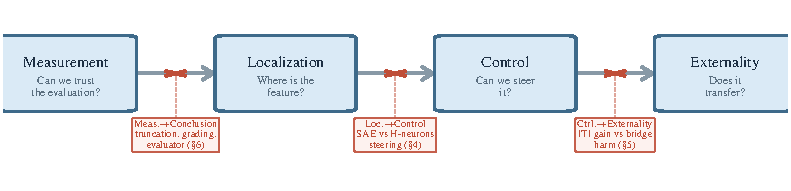
\includegraphics[width=\textwidth]{figures/fig1_scaffold.pdf}
  \caption{The Four-Stage Interpretability Scaffold and three empirical gates. Stages run left to right; each transition is a question the next stage assumes has been answered. Three gates mark where the readout-to-steering heuristic broke in our case study: one \emph{within-stage} (Measurement$\to$Verdict, \S\ref{sec:measurement}: grading shifted the verdict, while output-length checks and the evaluator audit exposed residual measurement risk and rubric dependence) and two \emph{inter-stage} (Localization$\to$Control, \S\ref{sec:localization}; Control$\to$Externality, \S\ref{sec:externality}). Within-stage gates tether to a stage box; inter-stage gates tether to the transition arrow.}
  \label{fig:scaffold}
\end{figure*}

\textbf{Contributions.}
(1)~A readout-to-control audit: a Gemma FaithEval comparison showing that similar held-out readout quality for H-neurons and SAE features can yield sharply different behavioral outcomes under matched surface evaluation.
(2)~A within-SAE selector audit: a Gemma candidate-pool ablation showing that readout, prompt-end utility, and answer-span utility selectors produce different margin effects while all miss the compliance endpoint.
(3)~A control-to-externality audit: an ITI study showing that TruthfulQA MC gains do not license open-generation claims, with a bridge failure taxonomy dominated by wrong-entity substitution.
(4)~A measurement audit: a jailbreak evaluation showing that scoring granularity changes verdicts, with output-length exposure and evaluator construct choices retained as reporting risks.
(5)~A claim-discipline framework: a four-gate checklist for reporting activation-steering claims.

\textbf{Study orientation.}
This paper is a single-model comparative case study in Gemma-3-4B-IT \citep{gemma2025}.
We compare multiple intervention families (neuron scaling, SAE feature steering, and inference-time intervention via attention heads) across contextual faithfulness (FaithEval \citep{ming2025faitheval}), answer selection (TruthfulQA \citep{lin2022truthfulqa}), open-ended factual generation (TriviaQA \citep{joshi2017triviaqa}, SimpleQA Verified \citep{haas2025simpleqaverified}), domain QA (BioASQ \citep{tsatsaronis2015bioasq}), and jailbreak settings (JailbreakBench \citep{chao2024jailbreakbench}).
All claims are surface-specific: FaithEval is a context-faithfulness / anti-compliance surface, TruthfulQA MC constrained answer selection, TriviaQA bridge and SimpleQA Verified open-ended factual generation, and JailbreakBench a harmfulness-evaluation surface.
Within that scope, the paper asks three bounded empirical questions:
(1)~Is held-out readout quality enough to select steering targets? (\S\ref{sec:localization})
(2)~Do answer-selection gains transfer to open-ended factual generation? (\S\ref{sec:externality})
(3)~Do plausible measurement choices leave the jailbreak verdict stable? (\S\ref{sec:measurement})
These surface-specific questions do not claim a new steering method or a general failure of detector-based targets.
Appendix stress tests on \texttt{Mistral-Small-24B-Instruct-2501} and SIMID diagnostic artifacts are used only as failed or incomplete gates.

% ======================================================================
% 2. RELATED WORK
% ======================================================================
\section{Related Work}
\label{sec:related}

Foundational probe critiques establish that high readout accuracy can arise for reasons the model does not functionally rely on \citep{hewitt2019control,elazar2021amnesic,kumar2022probes}. The linear representation hypothesis \citep{park2024linear} makes the complementary positive prediction that concepts encoded as linear directions should support both detection and control, which the present paper probes empirically. \citet{hase2023localization} provide a close editing precedent: better localization need not predict better control.

The steering lineage motivating this audit runs from representation engineering and activation addition \citep{zou2023repe,turner2024steering} through ITI \citep{li2023iti}. Within SAE-based interventions, foundational feature work \citep{cunningham2023saes} and the Gemma Scope release \citep{lieberum2024gemmascope} make sparse features available at scale, while target-selection studies show that not all salient features steer well: high-scoring SAE features need not control behavior \citep{arad2025saes}, detection and steering need not be jointly optimized \citep{wu2025axbench}, \citet{wang2026interpretability} report only a weak positive association between SAE interpretability and steering utility across 90 SAEs (Kendall's $\tau_b \approx 0.298$), and \citet{bhalla2024unifying} describe a predict/control discrepancy for interpretability-based interventions.

Transfer and reliability work narrows the claim space further. \citet{li2023iti} already showed that ITI's multiple-choice gains can diverge from generative gains; \citet{tan2024steering} study the brittleness and input sensitivity of steering vectors; \citet{pres2024reliable} show that behavior-steering evaluations can be format-dependent; and \citet{opielka2026causality} show that causally effective vectors can still be surface-specific. Positive counterexamples remain important: refusal directions and targeted multi-attribute steering can work when the behavioral target is better matched to the intervention \citep{arditi2024refusal,nguyen2025matsteer}.

Measurement fragility is a parallel reviewer concern. JailbreakBench \citep{chao2024jailbreakbench} provides the benchmark surface used here; StrongREJECT \citep{souly2024strongreject} showed that binary scoring can overestimate jailbreak effectiveness; \citet{chen2025safer} and \citet{eiras2025judge} show that evaluator artifacts and rubric choices matter; and \citet{huang2025guidedbench} argue that guideline-conditioned judging can materially change jailbreak conclusions.
For factuality more directly, \citet{yona2026metacognition} argue that hallucination mitigation should report utility-error tradeoffs and spillover costs alongside calibration or single operating points; our SimpleQA and bridge analyses instantiate those cautions for activation interventions.

Concurrent SAE-centric analyses \citep{arad2025saes,wang2026interpretability} and synthetic-benchmark evaluations \citep{wu2025axbench} make detection/control divergence increasingly clear within single-family settings.
The core contribution here is a cross-representational FaithEval comparison: neurons and SAE features are evaluated on the same real behavioral surface with closely matched held-out readout quality.
Two supporting additions broaden that case study.
First, on TriviaQA bridge generation we provide a frozen-protocol behavioral diagnosis of the transfer failure, where wrong-entity substitution is the most common manually coded right-to-wrong pattern and formal refusal is rare.
Second, we show that scoring granularity can change the verdict for the same representation-engineering intervention outputs, while output-length checks and a held-out evaluator audit reveal residual measurement risk.
We synthesize these observations in a four-stage audit framework (measurement, localization, control, externality).

% ======================================================================
% 3. LOCALIZATION -> CONTROL
% ======================================================================
\section{Similar Readout Quality Does Not Guarantee Control}
\label{sec:localization}

\subsection{The Readouts Are Real}

The intervention targets were selected through held-out predictive readouts.
A sparse H-neuron probe following \citet{gao2025hneurons} identified 38 positive-weight neurons out of 348,160 feed-forward neurons and achieved AUROC~$0.843$ (accuracy 76.5\%, $n_{\text{test}} = 780$).
A parallel L1 probe on Gemma Scope~2 SAE activations \citep{lieberum2024gemmascope} selected 266 positive-weight features across 10 layers and achieved AUROC~$0.848$ (accuracy 77.2\%, $n_{\text{test}} = 782$).
These are real held-out signals, though individual-weight interpretation remains fragile (Appendix~\ref{app:detector}).

\subsection{Comparable Readouts, Divergent Control}

Both methods achieve similar held-out detection quality, and we evaluate both interventions on the same 1,000 FaithEval items \citep{ming2025faitheval}.
The 38 probe-selected neurons were scaled multiplicatively across $\alpha \in \{0, 0.5, 1.0, 1.5, 2.0, 2.5, 3.0\}$, with $\alpha = 1.0$ as the no-op baseline.
The 266 tested Gemma Scope SAE features were scaled through an encode-modify-decode intervention on the same grid.

The neuron intervention showed a clear dose-response: compliance slope $+2.09$ pp/$\alpha$ $[1.38, 2.83]$, with perfect Spearman monotonicity ($\rho = 1.0$).
Relative to the no-op baseline, compliance at $\alpha = 3.0$ increased by $+4.5$~pp $[2.9, 6.1]$.
Across five unconstrained and three layer-matched random-neuron sets, all eight random seeds produced null slopes (maximum $+0.21$ pp/$\alpha$); every paired neuron-minus-random difference excluded zero.

The tested SAE intervention did not produce the same behavior.
The full-replacement H-feature slope was $+0.16$ pp/$\alpha$ $[-0.51, 0.84]$, with no monotonic trend ($\rho = 0.18$).
A delta-only architecture that cancels reconstruction error confirmed the null: delta-only H-feature slope $+0.12$ pp/$\alpha$, delta-only random-feature slope $-0.09$ pp/$\alpha$, both indistinguishable from zero.
The neuron baseline on the same three-alpha subset remained $+2.12$ pp/$\alpha$.

The paired neuron-minus-SAE slope difference was $+1.93$ pp/$\alpha$ $[+0.94, +2.92]$ (permutation $p < 0.001$).
On the same 1,000 FaithEval items, similar held-out readout quality did not predict intervention utility: H-neurons and SAE features showed comparable detector performance, yet only the neuron intervention produced a robust behavioral dose-response.

\paragraph{Within-SAE target-selection ablation.}
We next tested whether the SAE null could be explained by a poor target-selection rule.
The ablation used the same 509-feature Gemma SAE candidate set, the same extraction layers, and a single $\alpha = 0$ delta-only operator (feature zeroing) on a frozen $160/840$ validation/test FaithEval split.
The first ablation compared top-266 readout features, top-266 prompt-end validation-utility features, and ten layer-matched activation-weighted random zero-weight controls; all produced null compliance deltas on the $n = 840$ test split (all paired $95\%$ CIs include zero; point estimates $\le 0.72$~pp).
On the anti-compliance logprob margin, readout-selected features shifted the margin in the \emph{wrong} direction (+$0.92$~nats $[+0.61, +1.23]$ vs.\ no-op), while prompt-end utility-selected features reduced it by $-0.76$~nats $[-1.08, -0.42]$; the paired utility-minus-readout delta was $-1.68$~nats $[-2.17, -1.19]$.
Because both sides of that contrast share the same $\alpha = 0$ delta-only operator, any path artifact cancels; a dedicated path-drift control ($\alpha = 0$ on a single provably-dead zero-weight feature) independently moved the margin by only $+8.2\times 10^{-8}$~nats $[-2.4\times10^{-3}, +2.1\times10^{-3}]$.
A later answer-span selector on the same pool added a narrower finding: it reduced its native first-3-token answer-text margin ($-0.33$~nats $[-0.61, -0.06]$ vs.\ no-op), but left compliance null and underperformed the prompt-end utility selector on the original prompt-end margin ($+0.46$~nats $[+0.16, +0.75]$).
Within the same candidate pool, readout-, prompt-end-utility-, and answer-span-utility criteria therefore induce metric-specific margin effects, and no rule reaches the accuracy endpoint (Appendix~\ref{app:saeselector}).

\subsection{Synthesis}

H-neurons \emph{did} steer FaithEval compliance, and specificity was confirmed against eight matched random controls.
The refusal-direction literature \citep{arditi2024refusal} and targeted multi-attribute steering \citep{nguyen2025matsteer} are positive cases.
The narrower claim is that readout quality alone is an unreliable heuristic for predicting \emph{when} detection-based targets will steer behavior.
The tested SAE features matched H-neurons on the quantity most commonly used to justify steering (held-out AUROC) and missed the downstream behavioral endpoint.

A natural objection is that this comparable-readout design confounds representational basis with readout quality: SAE features and neurons differ in operator form, layer coverage, and feature granularity.
The within-SAE ablation above partly closes that gap: with operator form and the available extraction layers held fixed, readout-, prompt-end-utility-, and answer-span-utility selectors produce metric-specific margin effects, and none reaches the accuracy endpoint.
The remaining basis confound narrows the across-family inference, but readout quality alone did not suffice to predict steering utility in either the cross-representational comparison or within the SAE pool.
We discuss this limitation further in~\S\ref{sec:framework}.

\begin{figure*}[t]
  \centering
  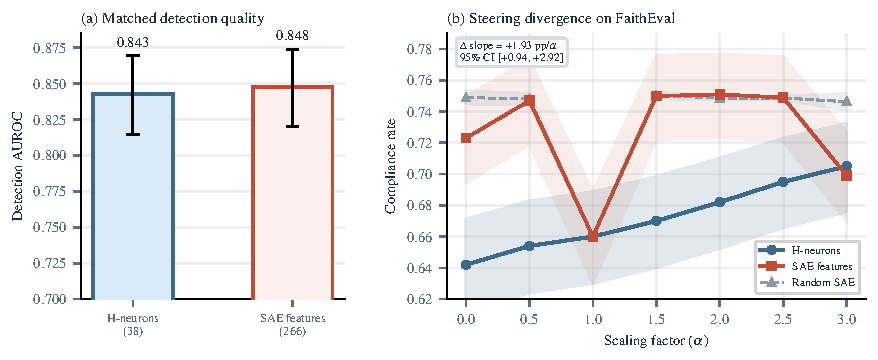
\includegraphics[width=\textwidth]{figures/fig2_matched.pdf}
  \caption{The anchor result: FaithEval comparable readouts, divergent control.
  (a)~H-neurons and SAE features have similar held-out detection AUROC.
  (b)~Only H-neurons produce a dose-dependent compliance increase; the tested SAE features and random SAE features show no reliable monotonic dose-response.
  The neuron-minus-SAE slope difference ($+1.93$ pp/$\alpha$, 95\% CI excludes zero) confirms the dissociation.}
  \label{fig:matched}
\end{figure*}

% ======================================================================
% 4. CONTROL -> EXTERNALITY
% ======================================================================
\section{Control Is Surface-Local and Can Externalize}
\label{sec:externality}

\subsection{Positive Results Are Task-Local}

Before testing transfer, we establish that detector-selected interventions can steer behavior on their primary surfaces.
H-neuron scaling (38 magnitude-ranked neurons) produces clear, dose-dependent effects on compliance-adjacent surfaces.
On FaithEval, compliance increases by $+4.5$~pp $[2.9, 6.1]$ above the no-op baseline at $\alpha = 3.0$ (slope $+2.09$ pp/$\alpha$), confirmed by 8-seed negative controls showing flat random-neuron baselines (mean slope $+0.02$ pp/$\alpha$).
On FalseQA \citep{hu2023falseqa} ($n = 687$), the same neurons show a dose-response slope of $+1.62$ pp/$\alpha$ $[0.52, 2.74]$.

However, the same 38 neurons show no robust net accuracy effect on BioASQ factoid QA \citep{tsatsaronis2015bioasq}: $-0.06$~pp $[-1.5, 1.4]$ on a well-powered sample ($n = 1{,}600$, MDE ${\sim}2$~pp), despite substantially perturbing answer style in 1,339 of 1,600 responses.
The flat accuracy endpoint coexists with substantial output perturbation, suggesting that behavioral activity and alias-accuracy movement come apart on this surface.
The intervention modulates compliance-adjacent behavior but does not improve domain-specific factual accuracy under the alias metric.

\subsection{ITI: Answer Selection vs.\ Open-Ended Generation}

ITI with directions fit from TruthfulQA multiple-choice contrasts \citep{lin2022truthfulqa} following \citet{li2023iti} improves answer selection.
At $\alpha = 8.0$, it yields $+6.3$~pp MC1 $[3.7, 8.9]$ and $+7.49$~pp MC2 $[5.28, 9.82]$ on held-out TruthfulQA folds, with 61 incorrect$\to$correct flips against 20 correct$\to$incorrect flips.

This MC/generation divergence echoes the tradeoff concern already visible in \citet{li2023iti}; here, SimpleQA Verified serves as a supporting stress test, while the locked bridge benchmark below is the main externality result.
The gain does not transfer to open-ended factual generation.
On a local copy of the 1,000-question SimpleQA Verified benchmark \citep{haas2025simpleqaverified}, graded with the benchmark's verified autorater, and with a prompt that removes the explicit escape hatch, ITI at $\alpha = 8.0$ reduces correct-answer rate from 4.6\% $[3.5, 6.1]$ to 2.8\% $[1.9, 4.0]$ (paired $\Delta = -1.8$~pp $[-3.1, -0.6]$).
The attempt rate collapses from 99.7\% to 67.0\%, while precision among attempted answers remains stable (${\sim}4$\%), suggesting epistemic caution without factual improvement.
Answer-selection success therefore provides no evidence for open-generation factual improvement, consistent with \citet{pres2024reliable} and \citet{opielka2026causality}.

\subsection{Bridge: Wrong-Entity Substitution}

The TriviaQA bridge benchmark \citep{joshi2017triviaqa} (held-out test set, $n = 500$, baseline adjudicated accuracy 45.0\%) provides the most informative externality result because it reveals a specific behavioral failure mode beyond the score drop.
The test set was evaluated under a one-shot frozen protocol: all parameters were locked from Phase~2 dev results, and no parameters were tuned on test data.

\textbf{The intervention changes outputs beyond suppression.}
At $\alpha = 8.0$, the baseline TruthfulQA-sourced ITI variant reduces adjudicated accuracy by $-5.8$~pp $[-8.8, -3.0]$ (CI excludes zero), with 43 right-to-wrong flips against 14 wrong-to-right rescues (net $-29$, McNemar $p = 0.0002$).
Both the primary (adjudicated) and floor (deterministic) accuracy deltas exclude zero, ruling out a grading artifact.

\textbf{Refusal is a minor part of the observed harm.}
NOT\_ATTEMPTED counts rise from 2 to 8, a small 1.2~pp effect.
Formal refusal accounts for 0 of 43 R$\to$W flips under the dual-rated coding.
The dominant damage is factual corruption.

\textbf{Wrong-entity substitution is the most common dual-rated failure mode.}
Entity-level factuality work treats wrong-entity substitution as a recognizable neighboring error family in generation \citep{nan2021entity}.
We use that literature only as adjacent taxonomy; it supplies no prior evidence for this exact steering failure mode.
Each of the 57 discordant test cases (43 R$\to$W + 14 W$\to$R) was coded by the first author and a blinded LLM judge (\texttt{gpt-4o-2024-11-20}, temperature 0, strict JSON schema) against a pre-registered four-category rubric whose decision rules were committed before any test label was appended.
Raw agreement was 96.5\% (Cohen's $\kappa = 0.90$, Gwet's AC1 = 0.96); the two disagreements were resolved under the pre-committed rule.
Of the 43 R$\to$W flips, 31 fell in the wrong-entity substitution category: the model replaces a correct factual answer with a different entity from the same semantic neighborhood ($31/43 = 72\%$; 95\% CI $[57, 83]$; Table~\ref{tab:substitution}).
The remaining 12 flips split into evasion/factual denial (9/43, 21\%), answer dilution (3/43, 7\%), and formal refusal (0/43).
This profile is consistent with a coarse behavior-level reweighting toward nearby wrong candidates; we treat it as a behavioral diagnosis without claiming an internal substitution circuit.
A teacher-forced gold-vs-wrong log-likelihood-margin check (Appendix~\ref{app:bridge_margin}) has the same directional R$\to$W/W$\to$R sign and no substitution-specific signature: non-substitution flips show larger compression than substitution flips.

The 14 wrong-to-right rescues show that the intervention is behaviorally active in both directions; all 14 are themselves coded as wrong-entity substitutions (Wilson 95\% CI $[78.5, 100]$), reinforcing the reweighting reading, and on this surface the damage rate is larger than the rescue rate.

\begin{table}[t]
\centering
\caption{Wrong-entity substitution examples from the TriviaQA bridge test set (E0 $\alpha\!=\!8$). The model swaps correct entities for semantically nearby incorrect ones.}
\label{tab:substitution}
\vskip 0.1in
\small
\begin{tabular}{@{}L{2.0cm}L{2.1cm}L{2.3cm}@{}}
\toprule
\textbf{Question} & \textbf{Baseline} & \textbf{ITI $\alpha\!=\!8$} \\
\midrule
Danny Boyle's 1996 ``Choose Life'' film? & Trainspotting & Slumdog M.\ (same director) \\
\addlinespace
Other musician with Buddy Holly and the Big Bopper in the Feb.\ 1959 crash? & Ritchie Valens & J.P.\ Richardson (same crash) \\
\addlinespace
Family Guy character who moved to Stoolbend, Virginia? & Cleveland Brown & Peter Griffin (same show) \\
\addlinespace
Dickens novel with Merdle, Sparkler, and Tattycoram? & Little Dorrit & Bleak House (same author) \\
\addlinespace
Comic whose June 1938 issue introduced Superman? & Action Comics & Detective Comics (same publisher) \\
\bottomrule
\end{tabular}
\vskip -0.1in
\end{table}

\begin{figure*}[t]
  \centering
  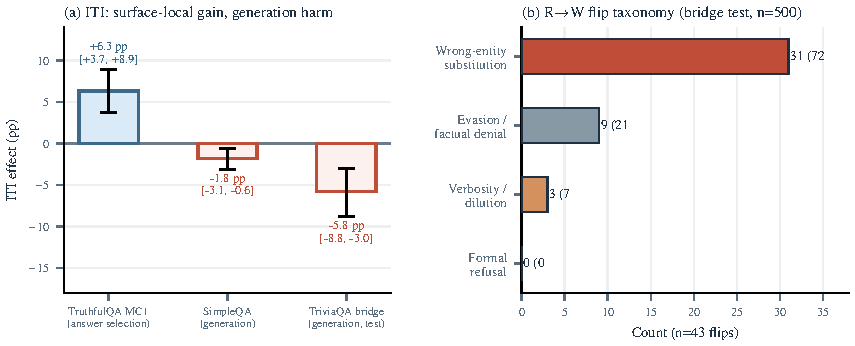
\includegraphics[width=\textwidth]{figures/fig3_bridge.pdf}
  \caption{Surface-local control and bridge failure modes.
  (a)~ITI improves TruthfulQA MC1 but harms both generation surfaces (CIs exclude zero).
  (b)~Among the 43 right-to-wrong flips on the TriviaQA bridge test set, wrong-entity substitution is the most common dual-rated failure mode ($72\%$; 95\% CI $[57, 83]$), with formal refusal rare.}
  \label{fig:bridge}
\end{figure*}

% ======================================================================
% 5. MEASUREMENT
% ======================================================================
\section{Measurement Choices Changed the Conclusion}
\label{sec:measurement}

The preceding sections established that detection quality does not predict steerability (\S\ref{sec:localization}) and that successful steering is narrow in scope (\S\ref{sec:externality}).
Both conclusions rest on behavioral measurements (jailbreak harmfulness rates, severity scores, and generation-surface accuracy) that are themselves products of evaluation choices.
In this section we show that those choices are part of the scientific result: scoring granularity shifted what we would have concluded about whether a given intervention worked on the same outputs, while output-length checks and the evaluator audit expose residual measurement risk on a held-out set.
The general point that evaluator choices matter is established (\S\ref{sec:related}); the specific finding here is that same-output measurement choices can reverse the conclusion about a representation-engineering intervention in the RepE sense \citep{zou2023repe}, even when two held-out evaluators tie in aggregate accuracy.

We organize the case study around the H-neuron jailbreak scaling experiment (38 probe-selected neurons, $\alpha \in \{0, 1, 1.5, 3\}$, $n = 500$ per condition), because its moderate effect size makes it sensitive to every measurement decision we examine.

\textbf{Output-length exposure remains a measurement risk.}
Short generation caps (e.g., 256 tokens) can bias intervention evaluations when steering changes response structure.
In our Gemma jailbreak audit, an archived 256-token run motivated a full-output rerun; that archived view is superseded and carries no claim-bearing effect.
The live Gemma result below is the same-output scoring-granularity contrast on the canonical full-output run.
The Mistral 2501 stress test in Appendix~\ref{app:mistral_stress} shows the scope condition: its 256-token diagnostic tracks full-output binary scoring much more closely, even though most rows are still truncated.
Output-length exposure is therefore a construct- and model-dependent measurement risk, and full-output scoring remains the safer reporting default.

\textbf{Scoring granularity changes the verdict.}
The same H-neuron jailbreak outputs look different under binary and graded evaluation.
A GPT-4o binary harmful/safe judge shows a $+3.0$~pp endpoint shift ($\alpha = 0 \to 3$, 152/500~$\to$~167/500), with a confidence interval that includes zero.
Under binary evaluation alone, the intervention looks weak and non-decisive.

A graded harmfulness rubric (CSV-v2) applied to the same outputs recovers a different result.
The H-neuron strict harmfulness slope is $+2.30$ pp/$\alpha$ $[+0.99, +3.58]$, while a matched random-neuron control is flat at $-0.47$ pp/$\alpha$ $[-1.42, +0.47]$.
The slope difference is $+2.77$ pp/$\alpha$ $[+1.17, +4.42]$ with permutation $p = 0.013$.
Binary scoring washes out this signal because the effect largely lives in the movement of borderline cases into clearer refusal or clearer compliance.

This is the section's core granularity result: binary evaluation suggests a weak or null effect; graded evaluation shows a positive dose-response.

\textbf{Evaluator dependence is part of the result.}
On a contamination-free 50-record holdout, four GPT-4o-based evaluators yield the accuracies in Table~\ref{tab:evaluator}.
No pairwise difference reaches statistical significance at $n = 50$.
CSV-v3 and StrongREJECT-GPT-4o both reach 96.0\% holdout accuracy with identical error sets.
We retain CSV-v3 for its richer outcome taxonomy without claiming accuracy superiority.

The residual disagreement is informative because it clusters on a recognizable response type: refuse-then-comply outputs.
StrongREJECT's formula zeroes the final score when \texttt{refused = 1}, even if later text contains specific harmful substance.
We therefore treat evaluator disagreement as construct pluralism \citep{eiras2025judge}.

\begin{table}[t]
\centering
\caption{Holdout evaluator accuracy (contamination-free split, $n = 50$). Prompt-clustered bootstrap 95\% CIs.}
\label{tab:evaluator}
\vskip 0.1in
\small
\begin{tabular}{@{}lcc@{}}
\toprule
\textbf{Evaluator} & \textbf{Accuracy} & \textbf{95\% CI} \\
\midrule
CSV-v3 (GPT-4o)     & 96.0\% & [90.0, 100.0] \\
StrongREJECT (GPT-4o) & 96.0\% & [90.0, 100.0] \\
CSV-v2 (GPT-4o)     & 92.0\% & [84.3, 98.0] \\
Binary judge (GPT-4o) & 90.0\% & [80.0, 98.0] \\
\bottomrule
\end{tabular}
\vskip -0.1in
\end{table}

% ======================================================================
% 6. FRAMEWORK & DISCUSSION
% ======================================================================
\section{A Four-Stage Audit Framework}
\label{sec:framework}

We distill the case study evidence into a practical audit for evaluating mechanistic intervention claims.
The audit has four stages: measurement, localization, control, and externality.
The stages record where intervention claims broke in this case study:

\begin{itemize}
  \item \textbf{Measurement$\to$Verdict.} Before deciding whether an intervention worked, one must trust the evaluation that defines the behavioral surface. In our jailbreak setting, binary-versus-graded scoring altered the conclusion about the same outputs, while output-length checks and the evaluator holdout exposed residual construct mismatch (\S\ref{sec:measurement}).
  \item \textbf{Localization$\to$Control.} A feature that predicts behavior on held-out data need not causally control that behavior when perturbed. SAE features matched H-neurons on detection quality, yet did not translate into useful control (\S\ref{sec:localization}).
  \item \textbf{Control$\to$Externality.} An intervention that succeeds on one surface may fail or cause harm on a nearby surface. ITI improved TruthfulQA MC1 but reduced open-ended factual accuracy, where wrong-entity substitution was the most common manually coded failure mode (\S\ref{sec:externality}).
\end{itemize}

Each stage transition is a distinct empirical claim.
Passing one does not license claims about the next.
Table~\ref{tab:checklist} summarizes the minimum evidence required at each gate.

\begin{table}[t]
\centering
\caption{Minimum audit for a credible steering claim.
A result that clears only one or two gates remains a monitoring or localization result; a control claim needs the control gate.}
\label{tab:checklist}
\vskip 0.1in
\small
\begin{tabular}{@{}L{1.8cm}L{5.0cm}@{}}
\toprule
\textbf{Gate} & \textbf{Evidence required} \\
\midrule
Measurement & Pre-specified metric; full-generation scoring when output length can alter labels; evaluator agreement check if intervention alters output style \\
\addlinespace
Localization & Held-out readout quality plus direct test of whether intervention through these components changes behavior \\
\addlinespace
Control & Dose-response on target surface; matched negative control (random component, random direction); effect size with CI \\
\addlinespace
Externality & At least one non-target surface; capability check; report harms and scope conditions explicitly \\
\bottomrule
\end{tabular}
\vskip -0.1in
\end{table}

In our reading of the recent steering literature, target-surface control is reported more often than matched negative controls, cross-surface tests, or evaluator audits.
In our case study, each omitted gate would have licensed a claim that the full audit rejects: without measurement audits, the jailbreak intervention looks null; without externality checks, the ITI intervention looks beneficial.
The checklist is an empirical codification of the points where our own conclusions changed.

\subsection{Five Recommendations}

\textbf{R1: Do not treat held-out readout quality as sufficient target-selection evidence.}
Metrics such as AUROC, accuracy, and probe coefficient magnitude are insufficient on their own for identifying useful steering targets.
Our comparison in \S\ref{sec:localization} shows that similar held-out AUROC can fail to predict intervention utility.

\textbf{R2: Validate on the behavioral surface you actually care about.}
Answer-selection benchmarks and open-ended generation benchmarks measure different constructs, and intervention effects do not transfer reliably between them (\S\ref{sec:externality}).

\textbf{R3: Use matched negative controls.}
When component search is large, post-hoc selection creates a multiple-comparisons problem.
Multi-seed random controls are necessary to establish that an effect is component-specific instead of a generic perturbation artifact.

\textbf{R4: Treat evaluator disagreement as information.}
When an intervention changes the surface form of outputs, different evaluators may reach different conclusions.
This disagreement reflects construct mismatch (\S\ref{sec:measurement}).

\textbf{R5: Report externality costs as first-class outcomes.}
Interventions that help on one metric can harm others.
Our bridge results show that the harm can be a specific, interpretable failure mode (\S\ref{sec:externality}).
Cross-surface effects belong next to the headline result.

\subsection{Limitations}

The primary claim-bearing experiments use a single model, Gemma-3-4B-IT.
Appendix~\ref{app:mistral_stress} reports stress tests on \texttt{Mistral-Small-24B-Instruct-2501}, but those results are failed or incomplete gates: FaithEval intervention is null, TruthfulQA MC1 fails its source-surface gate, and JailbreakBench has a large uncontrolled alpha curve.
The comparable-readout design keeps held-out AUROC close, although some other property of the feature family (operator form, layer coverage) could explain the steering divergence.
The within-SAE selector ablations reduce the target-selection concern but do not remove the cross-family operator-form confound.
SAE layer coverage is partial; a different SAE width or layer selection could yield non-null results.
The bridge failure-mode second rater is an LLM judge (GPT-4o).
Because it is not an independent human coder, we present the agreement reported in \S\ref{sec:externality} as a sensitivity check with limited force.
Jailbreak H-neuron specificity is single-seed ($p = 0.013$); matched multi-seed controls are needed before a stronger specificity claim.
SIMID remains diagnostic-only: historical open-label calibration failed the pre-specified kappa gate, and the partial prospective selected-TruthfulQA alpha 8 vs.\ 0 effect missed the primary effect gate while degrading same-scope MC accuracy and attempt rate.
Concurrent work \citep{wang2026interpretability,arad2025saes,wu2025axbench} already argues for interpretability/utility divergence from SAE-centric and benchmark-driven perspectives; we do not claim discovery of detector/control dissociation in general. Our distinctness lies in a stricter audit scaffold and a matched cross-representational comparison on a real behavioral surface.
The full limitation inventory is in Appendix~\ref{app:limitations}.

% ======================================================================
% 7. CONCLUSION
% ======================================================================
\section{Conclusion}

In Gemma-3-4B-IT, strong internal readouts supported monitoring and sometimes supported control.
Their usefulness as steering targets depended on the behavioral surface, the intervention operator, and the measurement procedure used to judge success.
The four-stage audit framework (measurement, localization, control, and externality) summarizes that bounded lesson: passing one gate does not license claims about the next.

% ======================================================================
% IMPACT STATEMENT
% ======================================================================
\section*{Impact Statement}

This paper presents work whose goal is to advance the field of Machine Learning, specifically evaluation methodology for safety-relevant model interventions.
The wrong-entity substitution failure mode documented here has implications for deployment of steering-based safety mitigations: interventions that appear beneficial on constrained evaluation surfaces may corrupt factual generation in ways that are harder to detect than outright refusal.

% ======================================================================
% REFERENCES
% ======================================================================
\bibliography{references}
\bibliographystyle{icml2026}

% ======================================================================
% APPENDIX
% ======================================================================
\newpage
\appendix

\section{Detector Interpretation Audits}
\label{app:detector}

The top-weight CETT neuron (L20:N4288) is not stable across regularization settings: it is absent at $C \le 0.3$, appears at $C = 1.0$, and drops to rank~5 at $C = 3.0$.
The extreme weight is better explained by L1 concentration among correlated features than by unique causal importance.
Additionally, full-response readouts are strongly length-confounded: response length dominates TruthfulQA-style signal by ${\sim}3.7\times$ under mean aggregation.
FaithEval uses single-letter extraction, so these audits leave the intervention claims intact while justifying the narrower wording in the main text.

\section{Construct Map}
\label{app:constructs}

\begin{table*}[t]
\centering
\caption{Benchmark construct map. Each evaluation surface measures a specific behavioral construct.}
\label{tab:constructs}
\vskip 0.1in
\small
\begin{tabular}{@{}L{2.5cm}L{5.0cm}L{2.3cm}L{4.2cm}@{}}
\toprule
\textbf{Benchmark} & \textbf{Construct} & \textbf{Primary Metric} & \textbf{Main Caution} \\
\midrule
FaithEval         & Context-resistance under anti-compliance prompting & Compliance rate & Context-faithfulness lever; no factual-QA claim \\
TruthfulQA MC1/2  & Answer selection under constrained candidates      & MC1 accuracy     & Does not measure open-ended generation \\
TriviaQA bridge   & Short-form factual generation                      & Adj.\ accuracy   & Dual-rated failure coding ($\kappa = 0.90$) \\
JailbreakBench    & Harmful compliance under adversarial prompting      & Graded harm rate & Binary eval.\ underpowered (MDE ${\sim}6$ pp) \\
BioASQ            & Domain-specific factoid QA (biomedical)             & Accuracy         & Flat despite behavioral perturbation \\
\bottomrule
\end{tabular}
\end{table*}

\section{FaithEval Detailed Rates}
\label{app:faitheval}

\begin{table}[ht]
\centering
\caption{FaithEval compliance by method and scaling factor ($n = 1{,}000$; Wilson 95\% CIs).}
\label{tab:faitheval_rates}
\vskip 0.1in
\small
\begin{tabular}{@{}cccc@{}}
\toprule
$\alpha$ & Neurons & SAE H-feat. & SAE rand. \\
\midrule
0.0 & 64.2\% & 72.3\% & 74.9\% \\
0.5 & 65.4\% & 74.7\% & 74.8\% \\
1.0 & 66.0\% & 66.0\% & 66.0\% \\
1.5 & 67.0\% & 75.0\% & 75.0\% \\
2.0 & 68.2\% & 75.1\% & 74.9\% \\
2.5 & 69.5\% & 74.9\% & 74.9\% \\
3.0 & 70.5\% & 69.9\% & 74.6\% \\
\bottomrule
\end{tabular}
\end{table}

\section{SAE Target-Selection Ablation on FaithEval}
\label{app:saeselector}

Section~\ref{sec:localization} briefly reported a within-SAE target-selection ablation; this appendix provides the numerical detail.

\paragraph{Design.}
Candidate pool: 509 SAE features with non-zero weight in the frozen FaithEval SAE classifier, drawn from the existing extraction layers $\{0, 5, 6, 7, 13, 14, 15, 16, 17, 20\}$ at $d_{\text{SAE}} = 16\,384$.
Stratified $160/840$ validation/test split by $(\text{num\_options}, \text{counterfactual\_key})$, seed~42, with $\text{validation} \cap \text{test} = \emptyset$.
Operator: SAE delta-only ablation at $\alpha = 0$ (encode $\to$ zero the target feature $\to$ decode $\to$ add the delta to the residual stream).
Three 266-feature selection rules are compared (readout: top probe weight; prompt-end utility: top validation reduction in the forced-choice anti-compliance margin; answer-span utility: top validation reduction in the first-3-token answer-text margin).
The utility and answer-span selectors each receive ten layer-matched zero-weight random seeds, sampled without replacement with weights proportional to validation-token activation rate via Efraimidis-Spirakis keys from a 112\,004-feature eligible pool.
A single-feature \emph{path-drift control} ($\alpha = 0$ on a layer-20 feature with zero classifier weight \emph{and} zero validation-token activation) isolates the residual contribution of routing through the SAE hook when the targeted feature is provably dead.

\paragraph{Results.} Table~\ref{tab:sae_selector} reports compliance and the two margin endpoints on the frozen $n = 840$ test split.

\begin{table*}[ht]
\centering
\caption{SAE target-selection ablation on FaithEval ($n = 840$). Margin contrasts are vs.\ no-op; lower margins are better because they reduce the misleading-vs-preferred logprob gap. CIs are 10\,000-sample paired bootstrap ($95\%$).}
\label{tab:sae_selector}
\vskip 0.1in
\footnotesize
\begin{tabular}{@{}L{4.3cm}L{2.1cm}L{4.2cm}L{4.2cm}@{}}
\toprule
\textbf{Family} & \textbf{Compliance} & \textbf{Prompt-end margin contrast} & \textbf{Answer-span margin contrast} \\
\midrule
No-op                     & $66.4\%$              & n/a & n/a \\
Readout-selected ($k{=}266$) & $66.0\%$           & $+0.92$ $[+0.61, +1.23]$ & $+0.65$ $[+0.30, +0.99]$ \\
Prompt-end utility-selected ($k{=}266$) & $66.2\%$ & $-0.76$ $[-1.08, -0.42]$ & $-0.10$ $[-0.30, +0.10]$ \\
Answer-span utility-selected ($k{=}266$) & $67.4\%$ & $-0.31$ $[-0.73, +0.12]$ & $-0.33$ $[-0.61, -0.06]$ \\
Path-drift ($k{=}1$ dead)  & $66.4\%$             & $+8.2{\times}10^{-8}$ $[-2.4{\times}10^{-3}, +2.1{\times}10^{-3}]$ & n/a \\
\bottomrule
\end{tabular}
\vskip -0.1in
\end{table*}

All selector families produce null compliance deltas (all paired $95\%$ CIs include zero; the answer-span selector's largest point estimate is $+0.95$~pp $[-0.83, +2.74]$ vs.\ no-op), so every tested selection rule misses the FaithEval accuracy endpoint.
On the prompt-end anti-compliance margin, readout-selected features shift the margin in the \emph{wrong} direction while prompt-end utility-selected features modestly improve it; the paired utility-minus-readout delta is $-1.68$~nats $[-2.17, -1.19]$.
This within-pool contrast is immune to path drift because both sides share the same $\alpha = 0$ delta-only operator; the explicit path-drift control ($+8.2\times 10^{-8}$~nats $[-2.4\times10^{-3}, +2.1\times10^{-3}]$) independently bounds invocation-only code-path drift far below the selection-specific effects.

A strictly-positive-utility augment ($k = 154$) guards against size-match dilution and reduces the margin by $-0.72$~nats $[-1.04, -0.39]$ vs.\ no-op, with three layer-matched random-positive seeds yielding paired deltas $-0.74$ $[-1.10, -0.36]$, $-0.81$ $[-1.16, -0.46]$, and $-0.42$ $[-0.75, -0.08]$~nats.
The ten-seed matched-random ensemble for the main bundle gives a seed-mean utility-minus-matched-random contrast of $-0.90$~nats (nested paired bootstrap $[-1.22, -0.56]$; naive seed bootstrap $[-1.17, -0.61]$); 9~of~10 seeds produce a negative paired delta.
The answer-span selector also improves over its own ten-seed matched-random null on its native margin (seed-mean $-0.53$~nats, nested $[-0.81, -0.26]$).
This is within-metric generalization from validation to test.
The more conservative cross-metric contrast is mixed, with answer-span selection worse than prompt-end utility selection by $+0.46$~nats $[+0.16, +0.75]$ on the original prompt-end margin.
The selector was frozen before any test labels were scored, and the random-null construction, the path-drift control, the 10-seed extension, and the answer-span extension were added sequentially in response to the adversarial audit flagged in our provenance notes.

\paragraph{Reading.}
Within the same candidate pool, readout-, prompt-end-utility-, and answer-span-utility criteria pick feature sets with metric-specific margin effects, and no rule reaches the accuracy endpoint.
The two intervention-aware $k=266$ sets share 167 features (Jaccard $0.46$), so the contrast is best read as evidence that the intervention objective is load-bearing within this pool.
It does not show that either objective discovers a behavioral steering handle.
The FaithEval SAE null is therefore robust to the tested readout-, utility-, and answer-span-selection rules within the available SAE extraction layers (L2 in Table~\ref{tab:limitations}).
Neither contrast elevates the SAE intervention to a successful steering handle; the margin-level separation between selection rules does not transfer to the behavioral endpoint.

\section{Benchmark Power Summary}
\label{app:power}

\begin{table}[ht]
\centering
\caption{Benchmark power and minimum detectable effect (MDE) summary.}
\label{tab:power}
\vskip 0.1in
\small
\begin{tabular}{@{}lccc@{}}
\toprule
\textbf{Benchmark} & $n$ & \textbf{Slope} & \textbf{MDE} \\
\midrule
FaithEval      & 1,000 & $+2.09$ pp/$\alpha$ & ${\sim}3$ pp \\
FalseQA        & 687   & $+1.62$ pp/$\alpha$ & ${\sim}4$ pp \\
JailbreakBench & 500   & $+2.30$ pp/$\alpha$ & ${\sim}5$ pp \\
BioASQ         & 1,600 & flat                & ${\sim}2$ pp \\
\bottomrule
\end{tabular}
\end{table}

\section{Bridge Margin-Shift Analysis}
\label{app:bridge_margin}

Section~\ref{sec:externality} reported the bridge wrong-entity-substitution taxonomy as a behavioral diagnosis.
This appendix quantifies the corresponding teacher-forced log-likelihood-margin shifts at the same intervention ($\alpha = 8$, $K = 12$, \texttt{first\_3\_tokens} decode scope) and states the supported and unsupported readings.

\paragraph{Design.}
For each case we sum per-token gold and wrong-entity logprobs over the first three continuation positions under baseline and ITI conditions, and report the per-case shift $\Delta_\text{margin} = \Delta_\text{ITI} - \Delta_\text{base}$, where $\Delta = \log p(\text{gold}) - \log p(\text{wrong})$.
Four cohorts: (A) $n = 31$ right-to-wrong (R$\to$W) wrong-entity substitutions; (B) $n = 12$ R$\to$W non-substitution flips (evasion/denial, dilution); (C) $n = 14$ wrong-to-right (W$\to$R) rescues; (D) $n = 200$ length-matched random wrong-entity controls drawn from unrelated bridge questions.
The analysis plan (endpoints, cohort partition, one-sided permutation direction) was sealed \emph{before} the full 257-case run executed; results are reported against that locked tree.

\begin{table}[ht]
\centering
\caption{Teacher-forced gold-vs-wrong log-likelihood-margin shift on the TriviaQA-bridge discordant set (first-$3$ tokens, ITI $\alpha = 8$ vs.\ baseline). Bootstrap $95\%$ CIs, 10\,000 resamples, seed~42.}
\label{tab:bridge_margin}
\vskip 0.1in
\small
\begin{tabular}{@{}lrrl@{}}
\toprule
\textbf{Cohort} & $n$ & $\Delta_\text{margin}$ & 95\% CI \\
\midrule
A: R$\to$W substitution     & 31 & $-10.16$ & $[-12.81, -7.60]$ \\
B: R$\to$W non-subst.       & 12 & $-40.06$ & $[-50.09, -30.37]$ \\
C: W$\to$R rescue           & 14 & $+4.73$  & $[+2.27, +7.25]$ \\
D: random control           & 200 & $-5.05$ & $[-6.55, -3.60]$ \\
\bottomrule
\end{tabular}
\vskip -0.1in
\end{table}

\paragraph{What holds.}
ITI causally compresses the gold-vs-wrong margin on R$\to$W cases and expands it on W$\to$R rescues, in the direction behavioral outcomes demand.
Substitution cases are significantly more compressed than length-matched random wrong-entity controls (A~$-$~D $= -5.10$~nats $[-8.22, -2.16]$, one-sided permutation $p = 0.0081$).

\paragraph{Unsupported reading.}
Non-substitution R$\to$W flips show \emph{larger} margin compression than substitution flips ($A - B = +29.90$~nats $[+19.91, +40.54]$; the substitution-specific prediction is formally reversed), concentrated but not exclusively at the first-token answer frame (position~0: $B = -21.74$~nats $[-29.48, -14.85]$ vs.\ $A = -3.49$~nats $[-5.14, -1.97]$).
The behavioral wrong-entity-substitution taxonomy ($\kappa = 0.90$) is therefore a reliable description of \emph{what} the model emits, while the log-likelihood analysis gives no distinct margin-shift signature for that taxonomy.
This refines the \S\ref{sec:externality} externality claim: the dominant-failure-mode statement is behavioral and interrater-defensible, and the margin analysis confirms ITI shifts probability mass in the predicted direction while changing the margin-level reading from substitution-specific entity suppression to answer-commitment margin compression on R$\to$W flips in general.

\section{Claim-Defense Ledger}
\label{app:claim_defense}

Table~\ref{tab:claim_defense} maps the main claim families to the exact metric-ledger IDs and source artifacts used to defend them.
It is a reviewer-facing index over existing measurements.

\begin{table*}[p]
\centering
\caption{Claim-defense ledger. IDs/artifacts anchor to \texttt{metric\_ledger.jsonl} and \texttt{surface\_crosswalk.jsonl}; brace notation expands prefixes; answer-span locators come from \texttt{heldout\_summary.json}.}
\label{tab:claim_defense}
\vskip 0.02in
\footnotesize
\setlength{\tabcolsep}{1pt}
\renewcommand{\arraystretch}{0.72}
\resizebox{0.86\textwidth}{!}{%
\begin{tabular}{@{}L{1.9cm}L{2.1cm}L{6.4cm}L{2.15cm}L{2.2cm}L{2.3cm}@{}}
\toprule
\textbf{Claim} & \textbf{Model / surface} & \textbf{Exact metric ID / source artifact} & \textbf{Estimator / CI} & \textbf{Gate status} & \textbf{Caveat} \\
\midrule
Comparable readouts &
Gemma-3-4B-IT / FaithEval readout &
\path|readout.disjoint.{auroc,accuracy}| / \path|classifier_disjoint_summary|;
\path|readout.sae.{auroc,accuracy}| / \path|classifier_sae_summary| &
Unpaired; stratified bootstrap for H-neuron readout; SAE point only. &
Localization / monitoring passed. &
L1; individual-weight interpretation remains fragile. \\

Gemma FaithEval H-neuron control &
Gemma-3-4B-IT / FaithEval anti-compliance, neuron scaling &
\path|intervention.faitheval.anti.{slope_pp_per_alpha,delta_noop_to_max_pp,delta_0_to_max_pp}| / \path|intervention_sweep_site|;
\path|intervention.faitheval.{random_mean_slope_pp_per_alpha,random_max_slope_pp_per_alpha}| / \path|faitheval_control_comparison| &
Paired bootstrap for slope / deltas; random summaries. &
FaithEval control and specificity passed. &
Surface-local compliance claim; no general factuality claim. \\

SAE H-feature null &
Gemma-3-4B-IT / FaithEval, tested Gemma Scope SAE operators &
\path|intervention.faitheval_sae.{h_slope_pp_per_alpha,neuron_minus_sae_slope_pp_per_alpha,permutation_p}| / \path|faitheval_sae_control_comparison|, \path|faitheval_sae_slope_difference| &
SAE slope summary; paired bootstrap gap; permutation test. &
SAE control gate did not pass; localization-to-control dissociation passed. &
L2 / L3 operator-form and layer-coverage limits. \\

Within-SAE selector defense &
Gemma-3-4B-IT / FaithEval, 509-feature SAE pool &
\path|intervention.faitheval_sae_utility.{utility_minus_noop_compliance_pp,utility_minus_noop_margin,utility_minus_readout_margin}| / \path|faitheval_sae_utility_selector_heldout|;
\path|heldout_summary.json::{heldout_answer_span_margin,heldout_compliance_answer_span_selected}| &
Paired bootstrap for compliance; continuous bootstrap for margins and answer-span locators. &
No selector reaches compliance endpoint. &
Margin-only, metric-specific, cross-metric mixed. \\

Surface-local H-neuron behavior &
Gemma-3-4B-IT / FalseQA and BioASQ, neuron scaling &
\path|intervention.falseqa.{slope_pp_per_alpha,delta_0_to_max_pp}| / \path|falseqa_results|;
\path|intervention.bioasq.{delta_0_to_max_pp,changed_response_count}| / \path|bioasq_results|, \path|bioasq_alpha_0_rows|, \path|bioasq_alpha_3_rows| &
Paired bootstrap for effects; paired response-join count for text change. &
FalseQA passes; BioASQ factual-accuracy endpoint fails / null. &
Alias and domain surface; no general factuality gain. \\

ITI MC vs. generation &
Gemma-3-4B-IT / TruthfulQA MC and SimpleQA open generation &
\path|transfer.truthfulqa_mc.{mc1.iti.delta_pp,mc2.iti.delta_pp}| / TruthfulQA ITI fold artifacts;
\path|transfer.simpleqa.{compliance_delta_0_to_8_pp,attempt_delta_0_to_8_pp}| / \path|simpleqa_ranked_results|, \path|simpleqa_alpha_0_rows|, \path|simpleqa_alpha_8_rows| &
Paired bootstrap on matched items / folds. &
MC answer-selection passed; open-generation transfer failed. &
MC / generation mismatch. \\

Bridge externality &
Gemma-3-4B-IT / TriviaQA bridge open generation, ITI &
\path|transfer.bridge.{adjudicated_accuracy_delta_pp,mcnemar_p,base_correct_iti_wrong,base_wrong_iti_correct}| / \path|bridge_phase3_site|;
\path|measurement.bridge_irr.{right_to_wrong.wrong_entity_substitution,cohen_kappa}| / \path|bridge_irr_summary| &
Report percentile CI; McNemar / flips; Wilson share; kappa. &
Externality failed and failure taxonomy accepted. &
L4 LLM second rater; wide Wilson interval. \\

Bridge margin boundary &
Gemma-3-4B-IT / TriviaQA bridge teacher-forced margins &
\path|transfer.bridge_margins.{a_rw_substitution.first3_shift_nats,b_rw_nonsubstitution.first3_shift_nats,c_wr_rescue.first3_shift_nats,a_vs_d.first3_shift_nats_gap,a_vs_d.first3_shift_nats_p}| / \path|bridge_margins_test_results| &
Paired within-cohort bootstrap; unpaired gap; permutation test. &
Broad margin sanity passed; substitution-specific mechanism failed. &
Behavioral diagnosis only. \\

Jailbreak measurement granularity &
Gemma-3-4B-IT / JailbreakBench, neuron scaling &
\path|intervention.jailbreak.binary.delta_0_to_max_pp| / \path|jailbreak_results|;
\path|measurement.jailbreak.v2.{h_slope_csv2_yes_pp_per_alpha,random_mean_slope_csv2_yes_pp_per_alpha,gap_h_minus_random_mean_pp_per_alpha,h_minus_random_permutation_p}| / \path|jailbreak_control_v2|, \path|jailbreak_seed0_control_audit| &
Binary paired bootstrap; graded v2 summaries; seed-0 permutation. &
Graded measurement detects signal; binary endpoint inconclusive. &
L5 single-seed specificity. \\

Evaluator holdout &
Gemma-3-4B-IT / JailbreakBench evaluator holdout &
\path|measurement.holdout.{csv2v3.accuracy,sr.accuracy,csv2v3_vs_sr_discordant_count,csv2v3_vs_sr_mcnemar_p,min_pairwise_mcnemar_p}| / \path|holdout_comparison| &
Cluster bootstrap by prompt ID; McNemar / discordance counts. &
No CSV-v3 superiority claim; construct-pluralism caveat retained. &
$n = 50$ holdout. \\
\bottomrule
\end{tabular}
}%
\end{table*}
\clearpage

\section{Second-Checkpoint and Diagnostic Stress Tests}
\label{app:mistral_stress}

Table~\ref{tab:mistral_simid_stress} records stress-test evidence that constrains the scope of the main Gemma claims.
These rows are excluded from the main story because each fails or lacks a required gate.
All Mistral rows use checkpoint \path|Mistral-Small-24B-Instruct-2501|.

\begin{table*}[ht]
\centering
\caption{Mistral and SIMID stress-test ledger. These artifacts constrain generalization; they do not upgrade the Gemma-local claims.}
\label{tab:mistral_simid_stress}
\vskip 0.05in
\footnotesize
\setlength{\tabcolsep}{2pt}
\renewcommand{\arraystretch}{0.88}
\resizebox{\textwidth}{!}{%
\begin{tabular}{@{}L{2.7cm}L{3.3cm}L{5.2cm}L{2.5cm}L{3.4cm}@{}}
\toprule
\textbf{Artifact} & \textbf{Model / surface} & \textbf{Evidence} & \textbf{Gate status} & \textbf{Caveat} \\
\midrule
Mistral sparse readout &
Mistral 2501 / TriviaQA-derived answer-token readout &
10 positive FFN targets; held-out accuracy $0.775$ $[0.715, 0.830]$ and AUROC $0.8711$ $[0.8185, 0.9172]$; source artifact \path|2026-04-29-mistral24b-cp23-pipeline-review.md|. &
Readout gate passed. &
Same-family 2501 checkpoint; no behavioral-control claim. \\
\addlinespace
Mistral FaithEval intervention &
Mistral 2501 / FaithEval, H-neuron scaling &
CP5 endpoint $\alpha=0 \to 3$ is $0.0$~pp $[-4.01, +4.00]$ with 9/9 paired flips; H1 C=0.75 endpoint is $+0.5$~pp $[-3.0, +4.0]$; source artifacts \path|2026-04-30-mistral24b-cp5-faitheval-review.md| and \path|2026-04-30-mistral24b-h1-c-sweep-review.md|. &
Control gate failed. &
Stress test supports gate discipline; FaithEval control gate remains failed. \\
\addlinespace
Mistral TruthfulQA MC &
Mistral 2501 / TruthfulQA MC, ITI &
MC1 moves 58/163 to 60/163, $+1.23$~pp $[-1.84, +4.29]$, McNemar $p=0.6875$; MC2 truthful mass moves $+1.91$~pp $[+0.50, +3.40]$; source artifact \path|2026-05-07-mistral24b-anchor2-truthfulqa-mc-review.md|. &
MC1 source gate failed. &
Wrapper stopped before bridge; no Mistral bridge externality claim. \\
\addlinespace
Mistral JailbreakBench curve &
Mistral 2501 / JailbreakBench, H-neuron scaling &
All judges have 2000/2000 valid rows. Endpoint $\alpha=0 \to 3$: binary-256 $+32.8$~pp, binary-full $+32.6$~pp, CSV-v3 $+32.4$~pp, StrongREJECT $+31.4$~pp. CSV-v3 and StrongREJECT agree on 91.8\% of rows ($\kappa=0.836$); source artifact \path|2026-05-06-mistral24b-anchor3-jailbreak-measurement-review.md|. &
Measurement curve present; specificity gate incomplete. &
No matched random or layer controls; 256-token diagnostic tracks full-output scoring in this run. \\
\addlinespace
SIMID diagnostic &
Gemma-3-4B-IT / SIMID selected TruthfulQA, ITI &
Historical calibration: 402 cases, raw agreement 91.5\%, Cohen's $\kappa=0.7594<0.8$. Partial prospective selected TruthfulQA alpha 8 vs.\ 0 open correctness is $+3.96$~pp $[-1.98, +9.91]$; MC letter accuracy is $-3.08$~pp $[-5.95, -0.66]$; attempt rate is $-8.59$~pp $[-13.44, -3.74]$. &
Calibration and effect gates failed. &
Diagnostic-only; no SIMID open-correctness or factuality-improvement claim. \\
\bottomrule
\end{tabular}
}%
\end{table*}

\section{Limitation Inventory}
\label{app:limitations}

\begin{table}[ht]
\centering
\caption{Key limitations and which claims they constrain.}
\label{tab:limitations}
\vskip 0.1in
\small
\begin{tabular}{@{}L{0.8cm}L{6.0cm}@{}}
\toprule
\textbf{\#} & \textbf{Limitation} \\
\midrule
L1 & Primary claim-bearing model is Gemma-3-4B-IT; Mistral stress tests exist but are failed or incomplete gates. \\
L2 & Matched-readout confound: the target-selection artifact form is addressed within the SAE pool (readout-, prompt-end-utility-, and answer-span-utility selectors give metric-specific margin effects with a null accuracy endpoint; Appendix~\ref{app:saeselector}); operator-form differences across families remain untested. \\
L3 & SAE layer coverage is partially addressed (selector searched all probe-nonzero features in the existing extraction layers); a different width or layer family could yield non-null results. \\
L4 & Bridge failure-mode second rater is an LLM judge (GPT-4o), with raw agreement 96.5\% ($\kappa = 0.90$, AC1 = 0.96) and limited force as an IRR check. \\
L5 & Gemma JailbreakBench H-neuron specificity is single-seed ($p = 0.013$); stronger specificity requires matched multi-seed controls. \\
L6 & Mistral Anchor 3 shows a large JailbreakBench alpha curve across judges, but it lacks matched random and layer controls. \\
L7 & SIMID historical and partial prospective artifacts failed the relevant calibration and effect gates, so they remain diagnostic-only. \\
\bottomrule
\end{tabular}
\end{table}

\end{document}
